\subsubsection{Förderband}
Da die Schwungräder durch den Abwurf um ca. 40\% (Berechnung in Formel \ref{equ_Prozentwert} im
Anhang) abgebremst werden, müssen sie nach jedem Wurf erneut auf die gewünschte Drehzahl
beschleunigt werden. Deshalb hat die Zuführung der Bälle in Abständen zu erfolgen. Weiter müssen die
einzelnen Tennisbälle immer mit der gleichen Geschwindigkeit bei den Schwungrädern eintreffen, damit
eine konstante Wurfweite entsteht. Die beste Art, beides zusammen zu realisieren ist ein Förderband.
Das Förderband wird zwischen den zwei Acrylglasplatten aufgespannt. Der Antrieb des Förderbandes
erfolgt mit einem DC-Motor. Dieser wird mit einem Verhältnis von $i=5:1$ untersetzt, um das benötigte
Drehmoment an die Antriebstrommel zu übertragen. Die Berechnungen dazu sind im Anhang in Formel
\ref{equ:M_Antrieb} ff. ersichtlich. Auf dem Förderband, welches aus einem
Flachbandriemen besteht, sind konvexe Führungsschaufeln angebracht. Diese sind so ausgerundet, damit
der Ball möglichst lange geführt werden kann und die Führungsschaufeln nicht in Berührung der
Schwungräder kommen. Die Schaufeln werden voraussichtlich mit dem Förderband verschweisst.
\begin{figure} [h!]
	\centering
	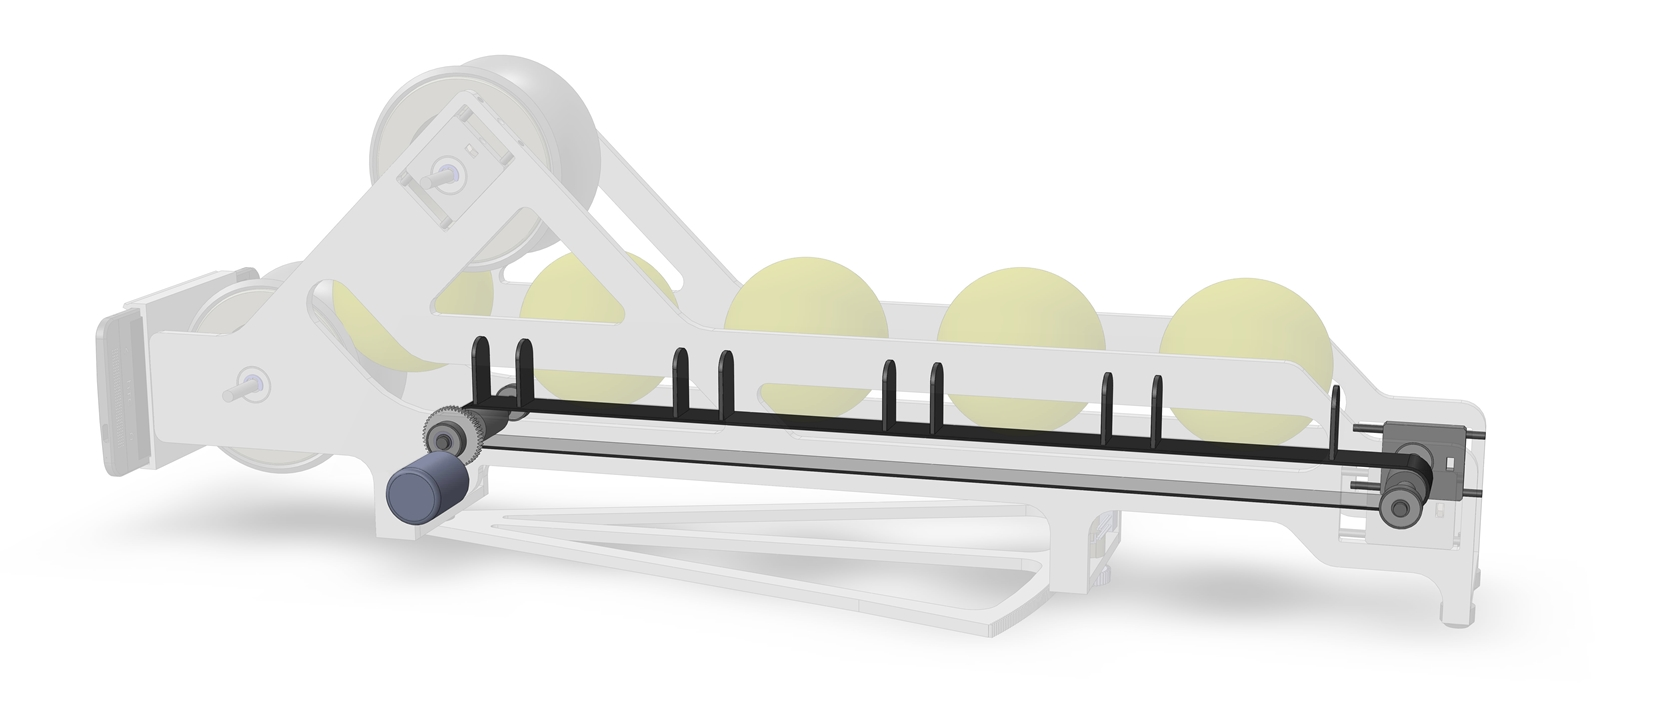
\includegraphics[width=0.9\textwidth,clip,trim=0mm 0mm 0mm 0mm]
	{Enddokumentation/Loesungskonzept/Bilder/Foerderband.jpg}
	\caption{Grafik Förderband}
	\label{fig:GrafikFörderband}	
\end{figure}
Aus Testversuchen der Ballzuführung wurde erkannt, dass für einen idealen Abwurf beide Räder
zeitgleich den Ball einklemmen müssen. Somit müssen die Bälle zunächst unterhalb des oberen
Schwungrades gefördert und anschliessend in einem 45$^\circ$ Winkel nach oben zugeführt werden. Dazu dient
ein Führungselement. Die Gestaltung dafür wird sich durch Tests zeigen. Als Ideen stehen zwei
Stangen oder ein Blech, welches die Bälle zu den Schwungrädern führt zur Auswahl. Die Abbildung
\ref{fig:GrafikFörderband} zeigt ein mögliche Ausführung der Schaufeln am Band.